\documentclass[a4paper,12pt]{article}
\usepackage{maratona_template}
\usepackage[T1]{fontenc}

\thispagestyle{empty}

\newtheorem{propriedade}{Propriedade}
\newtheorem{definicao}{Definição}

\begin{document}

\begin{center}
\begin{center}
  
\includegraphics[width=350]{figures/logo_if_horizontal.jpg}
\end{center}
\vspace{7cm}
\begin{center}
  
\includegraphics[width=\linewidth/2]{figures/logo_icpc_mdp.png}
\end{center}
\Large{Notebook para as Maratonas de Programação}\\
\large{Equipe SK Teletom}\\
\vspace{9cm}
\large{Versão 1.2 - Novembro 2018}
\end{center}

\newpage
\tableofcontents
\thispagestyle{empty}

\newpage
\section{Template}
\inserircodigo{c++}{template.cpp}{8}{8}{}

\newpage

\section{Matemática Computacional}

\subsection{Geometria Básica}
Vamos trabalhar com Geometria Euclidiana em 2D, em especial estaremos lidando com Geometria Analítica. Começaremos supondo que os estudantes entendem o conceito de ponto, reta e polígono simples. Agora vejamos alguns teoremas importantes:


\\~\\\noindent\textbf{Soma dos ângulos internos de um triângulo:}

\noindent A soma dos ângulos internos de triângulo é 180º

\\~\\\newline\noindent\textbf{Soma dos ângulos internos de um polígono:}

\noindent Vejamos que podemos triangular um polígono simples, basta escolhermos um dos pontos e ligá-los a todos os outros vemos então que teremos N - 2 triângulos, logo a soma dos ângulos internos será (N−2) \ang{180} graus.

\\~\\\newline\noindent\textbf{Teorema de Tales:}

\noindent Quando duas retas transversais cortam um feixe de retas paralelas, as medidas dos segmentos delimitados nas transversais são proporcionais. Por exemplo, usando a figura abaixo:

\begin{center}
  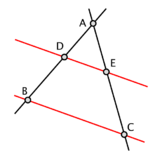
\includegraphics[width=\linewidth/4]{figures/matematica_computacional/geometria_basica/teorema_tales_1.png}
\end{center}

Então pelo teorema de Tales temos que:

\begin{center}
  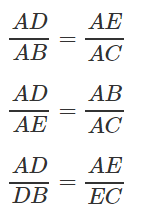
\includegraphics[width=\linewidth/5]{figures/matematica_computacional/geometria_basica/teorema_tales_2.png}
\end{center}

\\~\\\noindent\textbf{Teorema de Pitágoras:}

\noindent Um triângulo é retângulo se e somente se a soma dos quadrados de seus catetos (lados menores) for igual ao quadrado de sua hipotenusa (lado maior).
\\~\\
\noindent Na geometria analítica, nós consideramos que nossas figuras estão em um plano com dois eixos ortogonais que se cruzam na origem, esses eixos nos permitem definir coordenadas para os pontos dos planos e transformar um problema de geometria em um problema de álgebra, que computadores conseguem resolver.

\\~\\\noindent\textbf{Ponto:}

\noindentUm ponto em geometria analítica é apenas um par de números, suas coordenadas, uma horizontal e uma vertical.

\\~\\\noindent\textbf{Distância entre dois pontos:}

\noindentA distância entre dois pontos em geometria analítica pode facilmente ser descoberta usando o teorema de Pitágoras. Seja o primeiro ponto P1 (de coordenadas x1 e y1) e o segundo P2 (de coordenadas x2 e y2), então vemos que se construirmos um ponto P3 de coordenadas x2 e y1, teremos um triângulo retângulo, cuja hipotenusa é a distância entre P1 e P2, como mostra a figura abaixo:

\begin{center}
  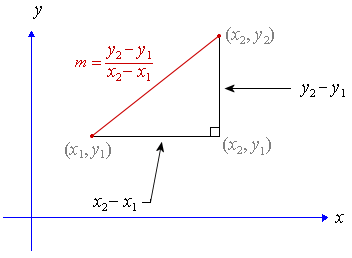
\includegraphics[width=\linewidth/2]{figures/matematica_computacional/geometria_basica/distancia_entre_dois_pontos_1.png}
\end{center}

Assim temos que a distância será:

\begin{center}
  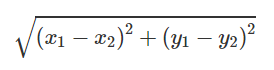
\includegraphics[width=\linewidth/3]{figures/matematica_computacional/geometria_basica/distancia_entre_dois_pontos_2.png}
\end{center}

\\~\\\noindent\textbf{Reta:}

\noindent Uma reta pode ser representada de várias formas, seguem aqui duas delas:

\begin{center}
  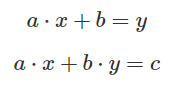
\includegraphics[width=\linewidth/4]{figures/matematica_computacional/geometria_basica/equacao_reta.png}
\end{center}

\noindent A primeira nos permite escrever uma coordenada dos pontos na reta em função da outra, sendo que a é chamado de coeficiente angular da reta (podemos ver facilmente que ele é a tangente do ângulo que a reta faz com o eixo horizontal), note que a e b são únicos. Já a segunda tem infinitas triplas a, b e c possíveis, porém se fixarmos o valor de um dos 3 os outros dois estão determinados, além disso essa forma tem a vantagem de nos permitir criar retas verticais, pois na forma anterior tais retas teriam a = infinito.

\\~\\\noindent\textbf{Círculo}

\noindent O circulo é o lugar geométrico dos pontos equidistantes a um dado ponto, chamamos esse ponto de centro e essa distância de raio. Dessa forma, vemos que se as coordenadas do centro são xc e yc, então todos os pontos obedecem a seguinte equação:

\begin{center}
  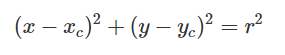
\includegraphics[width=\linewidth/3]{figures/matematica_computacional/geometria_basica/equacao_circulo.png}
\end{center}

\subsection{Geometria Computacional}
\noindent Essa clase de problemas em geral eles contêm códigos bastante complicados e podem ter certos problemas que geralmente não encontramos em outros tipos de questão, como por exemplo problemas com a precisão do float. Trabalharemos em 2D.

\\~\\\noindent\textbf{Ponto e Vetor:}

\noindent Pontos são geralmente representados por dois números reais, e são \textbf{análogos a um vetor indo da origem para onde o ponto fica}. Assim podemos criar um ponto de 3 formas: Pair:

\inserircodigo{c++}{matematica_computacional/geometria_computacional_basica/ponto_e_vetor_1.cpp}{8}{8}{}

Objeto:

\inserircodigo{c++}{matematica_computacional/geometria_computacional_basica/ponto_e_vetor_2.cpp}{8}{8}{}

Complex:

\inserircodigo{c++}{matematica_computacional/geometria_computacional_basica/ponto_e_vetor_complex.cpp}{8}{8}{}

\noindent O tipo complex de C++ já tem soma, subtração e multiplicação definidos para ele, porém deve-se tomar cuidado com esse tipo, pois o complex de int não é bem definido na std e vai variar com o compilador.

\noindent Agora exploremos algumas funções do complex antes de avançarmos:

\newline\noindent\textbf{real(p):} Retorna a parte real do número complexo p.
\newline\noindent\textbf{imag(p):} Retorna a parte imaginária do número complexo.
\newline\noindent\textbf{abs(p):} Retorna o comprimento do vetor (o valor absoluto de p)
\newline\noindent\textbf{sin(p), cos(p), tan(p):} São as funções trigonométricas no nosso número complexo.
\newline\noindent\textbf{arg(p):} Diz o ângulo que o vetor faz com a horizontal.
\newline\noindent\textbf{conj(p):} Retorna o conjugado do número complexo
\\~\\\noindent\textbf{Linhas:}

\noindent São simplesmente pares de pontos (não importando como você definiu o seu ponto).

\\~\\\noindent\textbf{Círculo}

\noindent Um círculo pode ser definido por seu centro e seu raio, desta forma temos que podemos definir um círculo como um pair de ponto e double.

\noindent Vejamos agora funções úteis nos problemas de geometria:

\\~\\\noindent\textbf{Produto Escalar}
\noindent O produto escalar é um dos dois tipos de produtos entre dois vetores e tem boas aplicações como veremos adiante. Vale lembrar que:

\begin{center}
  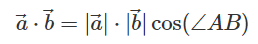
\includegraphics[width=\linewidth/4]{figures/matematica_computacional/geometria_computacional_basica/produto_escalar.png}
\end{center}

\inserircodigo{c++}{matematica_computacional/geometria_computacional_basica/produto_escalar.cpp}{8}{8}{}

\noindent Caso você tenha implementado o ponto com a complex também podemos definir o produto escalar da seguinte forma:

\inserircodigo{c++}{matematica_computacional/geometria_computacional_basica/produto_escalar_complex.cpp}{8}{8}{}

\noindent Supondo a e b não nulos, temos que o produto escalar deles vai ser menor que zero se eles tiverem um ângulo maior que 90º entre eles, igual a 0 se forem perpendiculares e maior que zero se formarem um ângulo agudo.

\\~\\\noindent\textbf{Produto vetorial:}

\noindent O produto vetorial geralmente tomaria dois vetores e nos retornaria um terceiro, porém aqui apenas nos importaremos com a magnitude do vetor retornado. Matematicamente temos:

\begin{center}
  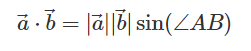
\includegraphics[width=\linewidth/4]{figures/matematica_computacional/geometria_computacional_basica/produto_vetorial.png}
\end{center}

\noindent E o código para calcular o produto vetorial é:

\inserircodigo{c++}{matematica_computacional/geometria_computacional_basica/produto_vetorial.cpp}{8}{8}{}

\noindent Ou ainda, se você estiver usando complex:

\inserircodigo{c++}{matematica_computacional/geometria_computacional_basica/produto_vetorial_complex.cpp}{8}{8}{}

\noindent O produto vetorial nos dá a área do paralelogramo com lados a e b (com sinal) e nos permite saber se o ângulo entre a e b é menor que 180 (se a área for menor que 0) , igual a 180 (se a área for igual a 0, no caso os vetores são paralelos), ou maior que 180 (se a área for maior que 180).

\noindent Agora por fim vejamos como essas funções nor permitem calcular quantias geometricamente importantes:

\\~\\\noindent\textbf{Distância entre dois pontos:}

\noindent A distância entre dois pontos é simplesmente o módulo do vetor que liga esses pontos, dessa forma basta subtrairmos um ponto do outro e retornarmos o módulo da resultante:

\inserircodigo{c++}{matematica_computacional/geometria_computacional_basica/distancia_entre_dois_pontos.cpp}{8}{8}{}

\noindent Usando a complex podemos escrever:

\inserircodigo{c++}{matematica_computacional/geometria_computacional_basica/distancia_entre_dois_pontos_complex.cpp}{8}{8}{}

\\~\\\noindent\textbf{Distância entre ponto e reta:}

\noindent A distância de um ponto para uma linha é igual a distância do ponto a um ponto qualquer da linha vezes o ângulo que esse vetor faz com a linha, assim podemos usar o produto vetorial para conseguir essa distância:

\inserircodigo{c++}{matematica_computacional/geometria_computacional_basica/distancia_entre_ponto_e_reta.cpp}{8}{8}{}

\\~\\\noindent\textbf{Área do Polígono}

\noindent Uma fórmula conhecida para a área de polígonos é a shoelace formula (muito usada em geometria analítica). Assim, sendo um polígono um vector de pontos ordenados tais que dois pontos adjacentes são uma aresta:

\inserircodigo{c++}{matematica_computacional/geometria_computacional_basica/area_do_poligono.cpp}{8}{8}{}

\\~\\\noindent\textbf{CCW}

\noindent A última função interessante que veremos toma 3 números e retorna se eles formam um ângulo convexo ou côncavo.

\inserircodigo{c++}{matematica_computacional/geometria_computacional_basica/ccw.cpp}{8}{8}{}

\noindent Note que em alguns juízes, e na OBI, muitas vezes erros de precisão podem levar um algoritmo correto a receber um \textbf{WA} (resposta errada), nesse caso não se deve usar a \textbf{complex} e sim um \textbf{pair} de \textbf{long long int} ou uma \textbf{struct}, e todas as operações que envolverem igualar duas frações, a/b e c/d, devem ser checados do seguinte modo:

\inserircodigo{c++}{matematica_computacional/geometria_computacional_basica/comparacao_fracoes.cpp}{8}{8}{}



\subsection{Primos}

\subsubsection{Primo rápido – O($\surd$n)}

\inserircodigo{c++}{matematica_computacional/primo_rapido_sqrt_n.cpp}{8}{8}{}

\subsubsection{Crivo de Erastótenes}
\indent Dados N e Q, com ambos menores que $10^6$, teremos Q inteiros a, menores N, e devemos responder para cada um deles se ele é primo.
\inserircodigo{c++}{matematica_computacional/crivo_erastotenes.cpp}{8}{8}{}

\subsubsection{Fatoração de primos}
A fatoração de números primos transforma um número grande em um produto de primos. Por exemplo, 5733, a fatoração pode transformá-lo em 3x3x7x7x13.

\inserircodigo{c++}{matematica_computacional/fatorizacao_primos.cpp}{8}{8}{}

\subsubsection{Números primos menores que 100}

// there are 25 numbers\newline
2, 3, 5, 7, 11, 13, 17, 19, 23, 29, 31, 37,\newline
41, 43, 47, 53, 59, 61, 67, 71, 73, 79, 83, 89, 97

\subsection{Algoritmos de Euclides}
\subsubsection{Maior divisor comum – GCD}

\inserircodigo{c++}{matematica_computacional/maior_dc.cpp}{8}{8}{}

\subsubsection{Menor divisor comum – LCM}

\inserircodigo{c++}{matematica_computacional/menor_dc.cpp}{8}{8}{}

\subsubsection{Maior múltiplo comum – MMC}

\inserircodigo{c++}{matematica_computacional/mmc.cpp}{8}{8}{}

\subsection{Operadores binários}
\subsubsection{OR nos Bits ( | )}
\inserircodigo{c++}{matematica_computacional/or_nos_bits.cpp}{8}{8}{}

\subsubsection{AND nos bits (\&)}
\inserircodigo{c++}{matematica_computacional/and_nos_bits.cpp}{8}{8}{}

\subsubsection{XOR nos bits (\textsuperscript{$\wedge$})}
\inserircodigo{c++}{matematica_computacional/xor_nos_bits.cpp}{8}{8}{}

\subsubsection{Shift Esquerdo ( << )}
\inserircodigo{c++}{matematica_computacional/shift_esq.cpp}{8}{8}{}

\subsubsection{Shift Direito ( >> )}
\inserircodigo{c++}{matematica_computacional/shift_dir.cpp}{8}{8}{}

\subsection{Manipulação de bits}
\subsection{Checar se um dado bit está ligado}
\inserircodigo{c++}{matematica_computacional/check_bit_is_set.cpp}{8}{8}{}

\subsection{Extrair o bit menos significante}
\inserircodigo{c++}{matematica_computacional/get_lsb.cpp}{8}{8}{}

\subsection{Contar o número de bits iguais a 1}
\inserircodigo{c++}{matematica_computacional/contar_bits_iguais_1.cpp}{8}{8}{}

\subsection{Checar se um número é potência de 2}
\inserircodigo{c++}{matematica_computacional/check_is_power_2.cpp}{8}{8}{}

\subsection{Ligar um bit em um número}
\inserircodigo{c++}{matematica_computacional/liga_bit_em_numero.cpp}{8}{8}{}

\subsection{Desligar o bit}
\inserircodigo{c++}{matematica_computacional/desliga_bit.cpp}{8}{8}{}

\subsection{Módulo de $2^{i}$ usando bitwise}
Para realizar o módulo de $2^{i}$, ( 2, 4, 8, 16 ...)

\inserircodigo{c++}{matematica_computacional/modulo_2i_bitwise.cpp}{8}{8}{}

\subsection{Divisão de números inteiros com resto negativo}

Caso seja necessário dividir números inteiros com resto um resto que possivelmente negativo

\inserircodigo{c++}{matematica_computacional/div_numeros_inteiros_resto_negativo.cpp}{8}{8}{}

\subsection{Condição existência e classificação de triângulo}

Para um triângulo existir, as três condições devem ser satisfeitas.

\inserircodigo{c++}{matematica_computacional/condicao_existencia_triangulo.cpp}{8}{8}{}

\subsection{Comparação entre 2 valores tipo Double}

A comparação entre dois doubles pode retornar valores indejados. Por isso uma função especial para comparação pode ser necessária.

\inserircodigo{c++}{matematica_computacional/comparacao_double.cpp}{8}{8}{}

\subsection{Arredondamento para cima}

\inserircodigo{c++}{matematica_computacional/arrendondamento_cima.cpp}{8}{8}{}

\subsection{Número de casas decimais de um número}

\inserircodigo{c++}{matematica_computacional/num_casas_decimais_num.cpp}{8}{8}{}

\subsection{Zerar conteúdo de um array 2d}

\inserircodigo{c++}{matematica_computacional/zera_conteudo_array_2d.cpp}{8}{8}{}

\subsection{Zerar conteúdo de um array 1d}

\inserircodigo{c++}{matematica_computacional/zera_conteudo_array_1d.cpp}{8}{8}{}

\subsection{Cuidado para divisão de dois floats ou double}

\inserircodigo{c++}{matematica_computacional/div_float_double.cpp}{8}{8}{}

\subsection{Conversão inteiro para hexadecimal}

\inserircodigo{c++}{matematica_computacional/conversao_int_decimal.cpp}{8}{8}{}

\subsection{Adicionar notação cietífica}

\inserircodigo{c++}{matematica_computacional/adc_notacao_cient.cpp}{8}{8}{}

\subsection{Adicionar casas decimais fixas}

\inserircodigo{c++}{matematica_computacional/casas_decimais_fixas.cpp}{8}{8}{}

\subsection{Volume do cilindro}

\(pi * r2 * h\)

\subsection{Área Total}

\(A = Ab + Al = 2*\pi*r*(2+h)\) \newline
\(Ab = 2*\pi*r2\) \newline
\(Al = 2*\pi*r*h\)

\subsection{Somatório de Feynman}
Para saber quantos quadrados diferentes existem em um quadriculado de N x N quadrados \newline
\((n*(n+1)*((2*n)+1))/6\)

\subsection{Ponto de máximo e mínimo em uma parábola}
Se a < 0, ponto de máximo\newline
Se a > 0, ponto de mínimo

\begin{equation}
    x = \frac{-b}{2a}
\end{equation}
\begin{equation}
    x = \frac{\Delta}{4a}
\end{equation}

\subsection{Somatório de um intervalo [a,b] inclusivo}

\(((a + b) * (b - a + 1)) / 2\)

\subsection{Distância entre 2 pontos}

\(sqrt(pow((xf-xi),2) + pow((yf-yi),2))\)

\subsection{Conversão cartesiano para polar}

\( r = \)$\surd$\((a 2 + b2)\)\newline
\(\Phi = tg-1 b/a\)

\subsection{Conversão polar para cartesiano}

\( a = r cos ø\) \newline
\( b = r sem ø\)

\subsection{Número de permutações de um conjunto}

\inserircodigo{c++}{matematica_computacional/num_permutacoes_conj.cpp}{8}{8}{}

\subsection{Número de combinações de um conjunto}

\inserircodigo{c++}{matematica_computacional/num_combi_conj.cpp}{8}{8}{}

\subsection{Tricks do cmath}

\inserircodigo{c++}{matematica_computacional/tricks_cmath.cpp}{8}{8}{}

\subsection{Máximo entre dois números}

\inserircodigo{c++}{matematica_computacional/max_entre_dois_num.cpp}{8}{8}{}

\subsection{Mínimo entre dois números}

\inserircodigo{c++}{matematica_computacional/min_entre_dois_num.cpp}{8}{8}{}

\subsection{$A^b$ mod p}

\inserircodigo{c++}{matematica_computacional/ab_mod_p.cpp}{8}{8}{}

\subsection{n! mod p}

\inserircodigo{c++}{matematica_computacional/n_mod_p.cpp}{8}{8}{}

\subsection{Digital Root}
Vamos chamar o digital root de x como S(x). S(5) = 5, S(38) = S(3 + 8 = 11) = S(1 + 1 = 2) = 2, S(10) = S(1 + 0 = 1) = 1.
\subsubsection{Digital Root de um número X}
\inserircodigo{c++}{matematica_computacional/digital-root-x.cpp}{8}{8}{}

\subsubsection{K-ésimo número com Digital Root igual a X}
\inserircodigo{c++}{matematica_computacional/k-esimo-digital-root-igual-a-x.cpp}{8}{8}{}





\newpage
\section{Strings}

\subsection{Modificações}

\subsubsection{Dividir uma string de acordo com um token}

\inserircodigo{c++}{strings/modificacoes/dividir_string_por_token.cpp}{8}{8}{}

\subsubsection{Apagar um intervalo de uma string}

\inserircodigo{c++}{strings/modificacoes/apagar_intervalo_string.cpp}{8}{8}{}

\subsubsection{Remover um caracter de toda a string}

\inserircodigo{c++}{strings/modificacoes/remover_caractere_toda_string.cpp}{8}{8}{}

\subsubsection{Inverter String}

\inserircodigo{c++}{strings/modificacoes/inverter_string.cpp}{8}{8}{}

\subsubsection{Substring}

\inserircodigo{c++}{strings/modificacoes/substring.cpp}{8}{8}{}

\subsection{Verificações}

\subsubsection{Verificar se uma string está vazia}

\inserircodigo{c++}{strings/verificacoes/verifica_string_vazia.cpp}{8}{8}{}

\subsubsection{Verificar se caracter está entre [A-z]}

\inserircodigo{c++}{strings/verificacoes/verifica_caractere_intervalo_A_z.cpp}{8}{8}{}

\subsection{Conversões}

\subsubsection{String para int}

\inserircodigo{c++}{strings/conversoes/string_para_int.cpp}{8}{8}{}

\subsubsection{String para long long}

\inserircodigo{c++}{strings/conversoes/string_para_long_long.cpp}{8}{8}{}

\subsubsection{String para unsigned int}

\inserircodigo{c++}{strings/conversoes/string_para_unsigned_int.cpp}{8}{8}{}

\subsubsection{String para unsigned long long}

\inserircodigo{c++}{strings/conversoes/string_para_unsigned_long_long.cpp}{8}{8}{}

\subsubsection{Char para int}

\inserircodigo{c++}{strings/conversoes/char_para_int.cpp}{8}{8}{}

\subsubsection{Int para String}

\inserircodigo{c++}{strings/conversoes/int_para_string.cpp}{8}{8}{}

\subsubsection{Caracteres minúsculos}

\inserircodigo{c++}{strings/conversoes/caractere_minusculo.cpp}{8}{8}{}

\subsubsection{Caracteres maiúsculos}

\inserircodigo{c++}{strings/conversoes/caractere_maiusculo.cpp}{8}{8}{}

\subsection{Apagar um intervalo de uma string}
\inserircodigo{c++}{strings/modificacoes/apagar_intervalo_string.cpp}{8}{8}{}

\subsection{Remover um caracter de toda a string}
\inserircodigo{c++}{strings/modificacoes/remover_caractere_toda_string.cpp}{8}{8}{}

\subsection{Verificar se uma string está vazia}
\inserircodigo{c++}{strings/verificacoes/verifica_string_vazia.cpp}{8}{8}{}

\subsection{Inverter String}
\inserircodigo{c++}{strings/modificacoes/inverter_string.cpp}{8}{8}{}

\subsection{Criar uma nova string a partir de um intervalo de outra string}
\inserircodigo{c++}{strings/modificacoes/substring.cpp}{8}{8}{}

\subsection{Verificar se caracter está entre [A-z]}
\inserircodigo{c++}{strings/verificacoes/verifica_caractere_intervalo_A_z.cpp}{8}{8}{}

\subsection{Busca [A-z]}
\inserircodigo{c++}{strings/busca.cpp}{8}{8}{}

\subsection{Insert, Erase, Replace}
\inserircodigo{c++}{strings/insert_erase_replace.cpp}{8}{8}{}

\subsection{String Streams}
\inserircodigo{c++}{strings/string_streams.cpp}{8}{8}{}

\newpage
\section{Estruturas}
\subsection{Verificar se elemento existe em um vetor}
\inserircodigo{c++}{estruturas/verifica_se_elemento_existe_vector.cpp}{8}{8}{}

\subsection{Apagar elementos duplicados em um vetor}
\inserircodigo{c++}{estruturas/apagar_elementos_duplicados_vector.cpp}{8}{8}{}

\subsection{Ordenar vector forma crescente}
\inserircodigo{c++}{estruturas/ordenar_vetor_crescente.cpp}{8}{8}{}

\subsection{Ordenar vector forma crescente}
\inserircodigo{c++}{estruturas/ordenar_vetor_decrescente.cpp}{8}{8}{}

\subsection{Excluir primeiro elemento de um vetor}
\inserircodigo{c++}{estruturas/apagar_primeiro_elemento_vector.cpp}{8}{8}{}

\subsection{Excluir último elemento de um vetor}
\inserircodigo{c++}{estruturas/apagar_ultimo_elemento_vector.cpp}{8}{8}{}

\subsection{Alterar tamanho de um vector}
\inserircodigo{c++}{estruturas/alterar_tamanho_vector.cpp}{8}{8}{}

\subsection{Busca em um vetor}
\inserircodigo{c++}{estruturas/busca_vector.cpp}{8}{8}{}

\subsection{Busca em um vetor}
\inserircodigo{c++}{estruturas/busca_vector.cpp}{8}{8}{}

\subsection{Deque}
\indent Deque array dinâmico que funciona como vector mas, tem os métodos push\_front() e pop\_front().

\subsection{Definição de um pair}
\inserircodigo{c++}{estruturas/definicao_pair.cpp}{8}{8}{}

\subsection{Leitura de um pair}
\inserircodigo{c++}{estruturas/leitura_pair.cpp}{8}{8}{}

\subsection{Utilizando pair de pair}
\inserircodigo{c++}{estruturas/utilizando_pair_de_pair.cpp}{8}{8}{}

\subsection{Criando pair com dois valores}
\inserircodigo{c++}{estruturas/criando_pair_com_dois_valores.cpp}{8}{8}{}

\subsection{Fila}
\inserircodigo{c++}{estruturas/fila.cpp}{8}{8}{}

\subsection{Pilha}
\inserircodigo{c++}{estruturas/pilha.cpp}{8}{8}{}

\subsection{SET}
\inserircodigo{c++}{estruturas/set.cpp}{8}{8}{}

\subsection{Map}
\inserircodigo{c++}{estruturas/map.cpp}{8}{8}{}

\subsection{For em Map}
\inserircodigo{c++}{estruturas/for_em_map.cpp}{8}{8}{}

\subsection{Union-Find com PD}
\inserircodigo{c++}{estruturas/union-find-pd.cpp}{8}{8}{}

\subsection{Union-Find com PD que atualiza o tamanho dos conjuntos}
\inserircodigo{c++}{estruturas/union-find-pd-tamanho-conjunto.cpp}{8}{8}{}

\subsection{Fila de prioridades}
\inserircodigo{c++}{estruturas/fila_prioridades.cpp}{8}{8}{}

\subsection{Árvore de Segmentos}
\indent Encontra o valor mínimo em um interval em O(log n).
acao[i] representa o preço da ação de índice i
arvore[i] representa o valor contido no nó i da árvore.
\newline Ou seja, arvore[i] contém o índice da ação mais barata
no intervalo representado pelo nó i
(no) representa o nó que estamos na função recursiva o nó que estamos representa o segmento [i, j]
\newline A função coloca altera o valor da ação de índice (posicao) para (novo\_valor) e altera a árvore de acordo com o necessário
\begin{center}
  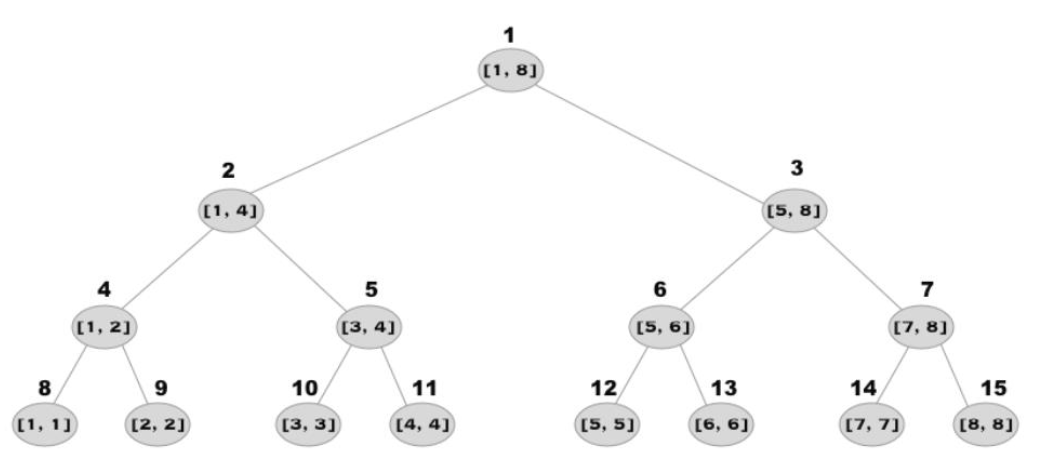
\includegraphics[width=\linewidth]{figures/estruturas/arvore_de_segmentos.png}
\end{center}
\inserircodigo{c++}{estruturas/arvore_segmentos.cpp}{8}{8}{}

\subsection{Árvore de Indexação Binária (BIT)}
\indent Dado um intervalo 1 a N. Permite adicionar valores aos elementos do intervalo e, efetuar o somatório de um intervalo intermediário entre 1 e N em O(log n).
\inserircodigo{c++}{estruturas/arvore_indexacao_binaria.cpp}{8}{8}{}

\subsection{Lazy Propagation}
\indent Você tem caixas N de frutas, númeradas de 1 a N, e duas possíveis operações.
\newline Operação 1: adicionar v frutas a cada uma das caixas de índice entre a e b(inclusive).
\newline Operação 2: responder quantas frutas existem nas caixas de índice entre a e b(inclusive).
\newline Com Lazy Propagation, uma adaptação que se faz na Árvore de Segmentos que permite fazer ambas as operações em O(log n) arvore[i] representa o valor contido no nó i da árvore.
\newline Ou seja, se o nó i representa o intervalo [X, Y], arvore[i] representa a soma das caixas de X a Y lazy[i] representa a soma de todas as operações atrasadas que devemos fazer ao nó i (no) representa o nó que estamos na função recursiva o nó que estamos representa o segmento [i, j] vamos somar (valor) a cada um dos índices no intervalo [a, b].
\inserircodigo{c++}{estruturas/lazy_propagation.cpp}{8}{8}{}

\subsection{Sort em structs}
\inserircodigo{c++}{estruturas/sort_em_structs.cpp}{8}{8}{}

\newpage
\section{Grafos}
\subsection{Representações de um Grafo}
\subsubsection{Matriz de Adjacência}

\indent\indent A matriz de adjacência consiste em saber, para cada possível par de vértices (u,v), se existe ou não a aresta (u,v).

\indent Vamos guardar na posição (i,j) da matriz a informação sobre a aresta (i,j). Podemos definir 0 para caso ela não existe e 1 para caso ela existe. No caso de termos um grafo com peso, podemos colocar o valor w na posição (i,j), onde w é o peso da aresta (i,j).

\indent Essa representação é fácil de implementar, mas sua complexidade de espaço é muito grande, equivalendo a O(N2), onde N é o número de vértices.

\indent Com relação ao tempo, podemos inserir e deletar uma aresta em O(1), mas saber quais são os vizinhos de um vértice custa O(N).

\indent A representação do grafo fica da seguinte maneira:

\begin{center}
  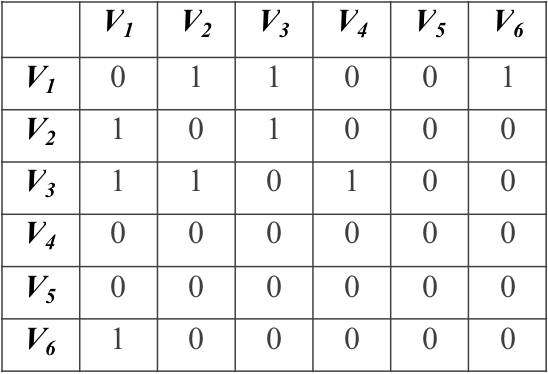
\includegraphics[width=\linewidth/2]{figures/grafos/representacao_matriz_adj.png}
\end{center}

\noindent Implementação em C++:

\inserircodigo{c++}{grafos/matriz_adjacencia.cpp}{8}{8}{}

\subsubsection{Lista de Adjacência}

\indent\indent A lista de adjacência se baseia em guardar, para cada vértice, quais são os seus vizinhos, ou, de uma maneira geral, guardar as arestas que partem desse vértice.

\indent O uso da lista de adjacência pode ser complicado de implementar e debugar para pessoas iniciantes, mas acaba sendo a representação mais usada por pessoas experientes. Isso se deve ao fato de a lista de adjacência possuir complexidade O(1) para inserir novas arestas e um tempo otimizado para consultas num único vértice.

\indent A representação do grafo por lista de adjacência fica da seguinte maneira:

\begin{center}
  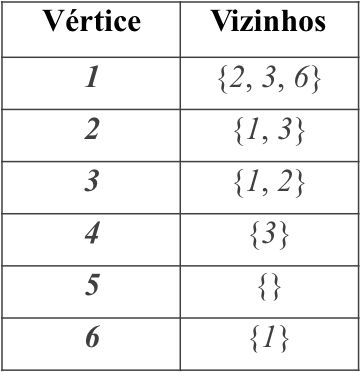
\includegraphics[width=\linewidth/2]{figures/grafos/representacao_lista_adj.png}
\end{center}

\noindent Implementação em C++:

\inserircodigo{c++}{grafos/lista_adjacencia.cpp}{8}{8}{}

\subsection{Lista de Arestas}
\inserircodigo{c++}{grafos/lista_de_arestas.cpp}{8}{8}{}

\subsection{Algoritmos}
\subsubsection{DFS(Busca em profundidade)}

Como o próprio nome já sugere, o algoritmo começa em um nó raiz e explora tanto quanto possível cada um dos seus ramos, antes de retroceder.

\inserircodigo{c++}{grafos/dfs.cpp}{8}{8}{}

\subsubsection{BFS(Busca em largura)}

\inserircodigo{c++}{grafos/bfs.cpp}{8}{8}{}

\subsubsection{Dijkstra - Caminho Mínimo entre dois pontos}

\inserircodigo{c++}{grafos/dijkstra.cpp}{8}{8}{"Lista de Adjacência"}
\inserircodigo{c++}{grafos/dijkstra_matriz.cpp}{8}{8}{"Matriz de Adjacência"}

\subsubsection{Kruskal - Árvore Geradora Mínima}

Conjunto de arestas com peso mínimo que ligam todo o grafo. \textbf{Para este algoritmo representar grafo utilizando lista de arestas.}

\inserircodigo{c++}{grafos/kruskal_agm.cpp}{8}{8}{}

\begin{center}
  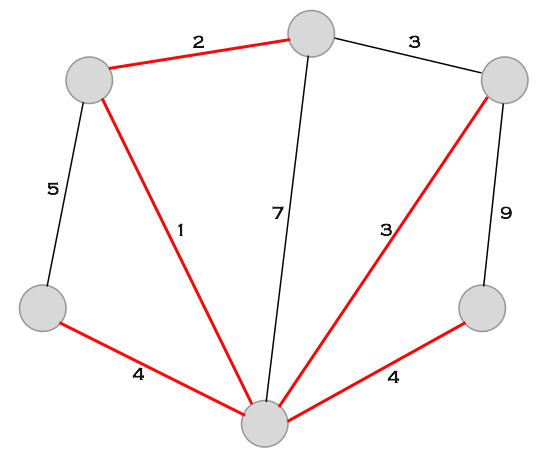
\includegraphics[width=\linewidth/2]{figures/grafos/agm.png}
\end{center}

\subsubsection{Prim - Árvore Geradora Mínima}

Algoritmo parecido com Dijkstra para encontrar árvore geradora mínima.

\noindent Implementação em C++:
\inserircodigo{c++}{grafos/prim_agm.cpp}{8}{8}{}

\subsubsection{Ordenação Topológica}

\textit{"Malter Warinho está ensinando seu filho a se vestir. Para isso, está dando instruções simples sobre a ordem em que seu filho deve se vestir para não colocar a roupa em ordem contrária (como o Superman). As instruções são do seguinte formato: as meias devem ser colocadas antes do sapatos; as calças devem ser vestidas antes do cinto; a camisa deve ser vestida antes do casaco; e por aí vai. Em alguns casos, não interessa a ordem em que deve ser colocada a roupa. Por exemplo, o filho pode colocar as calças antes do chapéu e vice-versa. Dada a lista de instruções e o número de peças de roupas, ajude o filho de Malter a se vestir."}\newline

\noindent Bem, para formalizar um pouco o problema, vamos montar um grafo direcionado onde:

\begin{itemize}
    \item cada vértice é uma peça de roupa.
    \item cada aresta partindo de um vértice X para um vértice Y significa que X tem que vir antes de Y.
\end{itemize}

\noindent Assim, pode se notar uma relação de transição: se X tem que vir antes de Y e Y tem que vir antes de Z, X tem que vir antes de Z.

\noindent Teremos então um grafo semelhante a este:

\begin{center}
  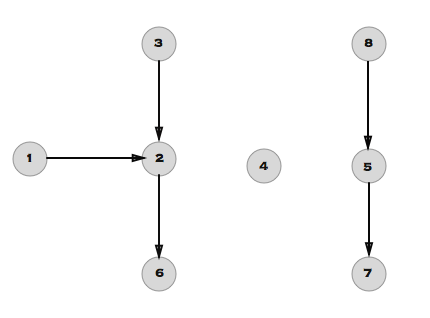
\includegraphics[width=\linewidth/2]{figures/grafos/OT.png}
\end{center}

\noindent Tendo uma noção do grafo, é fácil perceber alguns fatos simples:

\begin{itemize}
    \item se o grafo possui um ciclo, não há ordem em que se possa resolver o problema.
    \item podemos executar um vértice (vestir uma roupa) se, e somente se, todos os vértices (roupas) que possuem algum caminho até ele já foram executados.
\end{itemize}

\noindent Com apenas isso, já se pode pensar em um algoritmo bem simples para resolver o problema:

\begin{itemize}
    \item Pegar um vértice de grau de entrada zero (nenhuma aresta chega a ele) e acrescentar o vértice a ordem de execução.
    \item Remover todas as arestas que partem desse vértice e atualizar os graus dos vértices ligados a essas arestas.
    \item Repetir o processo até não haver mais vértices de grau de entrada zero (ou acabarem todos os vértices).
\end{itemize}

\noindent Se, ao final do processo, ainda sobrarem vértices, há um ciclo e não há ordem para resolver o problema. Caso contrário, o problema está resolvido.

\noindent Implementação em C++:
\inserircodigo{c++}{grafos/ordenacao_topologica.cpp}{8}{8}{}


\subsubsection{Floyd-Warshall - Menor Caminho}

Menor distância de qualquer vértice para qualquer outro.
\inserircodigo{c++}{grafos/floyd_warshall.cpp}{8}{8}{}


\subsubsection{LCA - Menor Ancestral Comum}

Ancestral comum mais próximo à dois vértices.

\begin{center}
  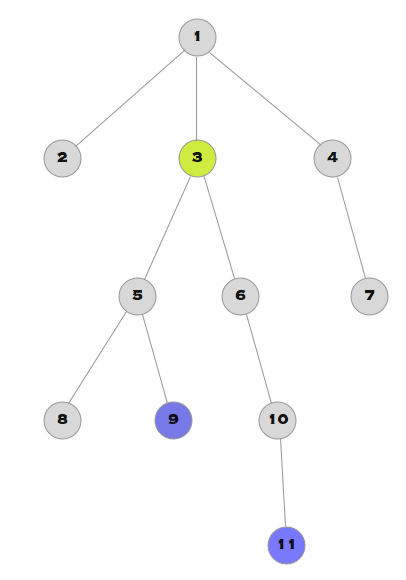
\includegraphics[width=\linewidth/2]{figures/grafos/LCA.png}
\end{center}

\inserircodigo{c++}{grafos/lca.cpp}{8}{8}{}

\subsubsection{Caminho Euleriano}

Um Caminho Euleriano de um grafo é um trajeto que passa por todas as arestas do grafo sem repetição.

\noindent\textbf{Existência:} Porém, antes de procurarmos um Caminho Euleriano para um grafo, precisamos saber se ele existe. Checar a existência de um Caminho Euleriano é, na verdade, bem fácil. Para um grafo ter um Caminho Euleriano, é suficiente e necessário satisfazer uma de duas condições:
\begin{itemize}
    \item Todos os vértices do grafo tem que ter grau par.
    \item Todos os vértices (ignorando-se os de grau zero) tem grau par, exceto dois vértices que possuem grau ímpar. Nesse caso, os dois vértices de grau ímpar são o início e o fim do Caminho.
\end{itemize}

\noindent Implementação em C++:

\inserircodigo{c++}{grafos/caminho_euleniano.cpp}{8}{8}{}

\subsubsection{Grafos bipartidos}
Um grafo é dito bipartido quando seus vértices podem ser divididos em dois conjuntos disjuntos tais que cada aresta ligue apenas vértices de grupos diferente.

\begin{center}
  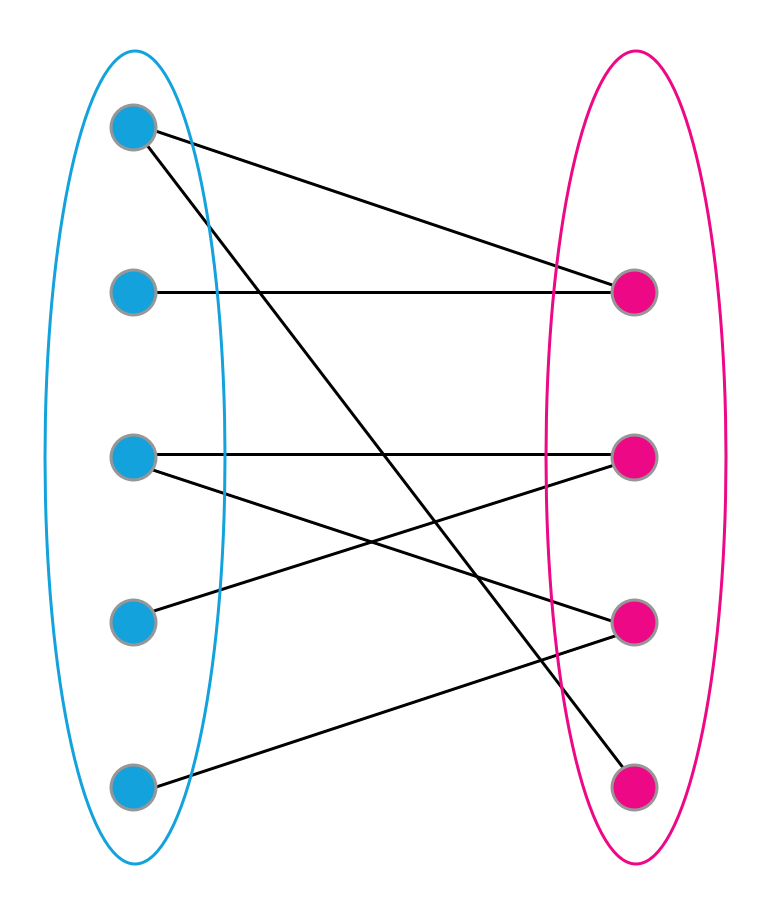
\includegraphics[width=\linewidth/2]{figures/grafos/grafos_bipartidos.png}
\end{center}

\noindent Implementação em C++:
\inserircodigo{c++}{grafos/grafo_bipartido.cpp}{8}{8}{}

\newpage

\section{Programação dinâmica}

\indent Aplicar a programação dinâmica se:

\begin{itemize}
    \item É possível dividir o problema em problemas menores.
    \item É possível encontrar as soluções ótimas para os subproblemas.
    \item Há sobreposição de subproblemas, isto é, há subproblemas que compartilham as mesmas respostas ótimas.
\end{itemize}

\subsection{Problema da mochila}

\indent O problema da mochila consiste de uma mochila de capacidade total $C$ e de $N$ itens que podem ser colocados dentro da mochila. Cada item possui um peso $p_i$ e um valor $v_i$. Objetiva-se colocar o maior número de itens dentro da mochila a fim de maximizar o valor total dos itens colocados. Matematicamente:

\begin{equation}
    \max \sum\limits_{i=1}^{I}v_i,
\end{equation}

\noindent onde $I$ é o conjunto de itens dentro da mochila. Sujeito as restrições:

\begin{equation}
    \sum\limits_{i=1}^{I}p_i \leq C
\end{equation}
\inserircodigo{c}{programacao_dinamica/mochila.c}{8}{8}{}

\subsection{Problema do troco}

\subsubsection{Problema do corte de hastes}

Dada uma haste de tamanho $n$ e o preço $p_i$ do corte de tamanho $i$. Qual é a melhor maneira de cortar a haste para maximizar o preço?

\inserircodigo{c}{programacao_dinamica/corte_haste.c}{8}{8}{}

\subsubsection{Dado valor e as moedas existe troco possível?}
\inserircodigo{c++}{programacao_dinamica/troco_eh_possivel.cpp}{8}{8}{}

\subsection{Calculadora Quebrada}
\inserircodigo{java}{programacao_dinamica/CalculadoraQuebradaUsandoPD.java}{8}{8}{}

\subsubsection{Mínimo de moedas para troco}
\inserircodigo{c++}{programacao_dinamica/minimo_moedas_troco.cpp}{8}{8}{}

\subsection{Contagem de inversões}

\indent Um dos problemas mais clássicos de programação é a contagem de inversões em uma sequência. De maneira simples, seja S = a1,a2,...,an. Uma inversão em S é um par (i,j), com i<j, tal que ai>aj. Sabendo disso, faça um programa que calcula o número de inversões em uma sequência S.

\inserircodigo{c++}{programacao_dinamica/contagem_inversoes.cpp}{8}{8}{}

\subsection{Maior Subsequência Comum}

\indent Dadas duas sequências s1 e s2, uma de tamanho n e outra de tamanho m, qual a maior subsequência comum às duas? Lembre-se que uma subsequência de s1, por exemplo, é simplesmente um subconjunto dos elementos de s1 na mesma ordem em que apareciam antes. Isto significa que {1, 3, 5} é uma subsequência de {1, 2, 3, 4, 5}, mesmo 1 não estando do lado do 3 na sequência original

\inserircodigo{c++}{programacao_dinamica/maior_subsequencia_comum.cpp}{8}{8}{}
\inserircodigo{c++}{programacao_dinamica/maior_subsequencia_comum_2.cpp}{8}{8}{}


\subsection{Maior Subsequência crescente}
Dada uma sequência s qualquer, descobrir o tamanho da maior subsequência crescente de s. Vale lembrar que uma subsequência de s é qualquer subconjunto de elementos de s. Veja, por exemplo:
s = {3, 4, 3, 5, 2, 7}
A maior subsequência crescente de s, neste caso é:
s' = {3, 4, 5, 7}
e tem tamanho 4.

\inserircodigo{c++}{programacao_dinamica/maior_subsequencia_crescente.cpp}{8}{8}{}

\subsection{Soma máxima em um intervalo}
\indent Dada uma sequência qualquer S=(s1,s2,s3,...,sn) qual a maior soma que podemos obter escolhendo um subconjunto de termos adjacentes de S? Se a sequência for, por exemplo, (1,-3,5,-2,1,-1), a soma máxima é 4, com os termos (5,-2,1).

\inserircodigo{c++}{programacao_dinamica/soma_maxima_intervalo.cpp}{8}{8}{}

\subsection{Vertex Cover}
\indent Um reino possui N cidades conectadas entre si por N − 1 rotas bidirecionais, onde se é possível viajar de qualquer cidade a qualquer outra. Preocupada com a segurança das rotas, a rainha decidiu instalar postos de seguranças em algumas cidades. O objetivo é que, para toda rota, exista um posto de segurança em ao menos uma das cidades conectadas por essa rota. Também preocupada com as finanças do reino, a rainha lhe contratou para selecionar achar o número mínimo de cidades em que é preciso construir um posto de segurança de forma a satisfazer as condições necessárias.

\inserircodigo{c++}{programacao_dinamica/vertex_cover.cpp}{8}{8}{}

\newpage

\section{Outros}

\subsection{Compilar programa em Java no CMD}
\noindent
javac NomeDoArquivo.java \newline
java NomeDaClasse

\subsection{Compilar programa em C++ no CMD}
\noindent
g++ arquivo.cpp \newline
a.exe < input.txt (No Windows) \newline
./a < input.txt (No Linux) 

\subsection{Tabela ASCII}
\begin{center}
  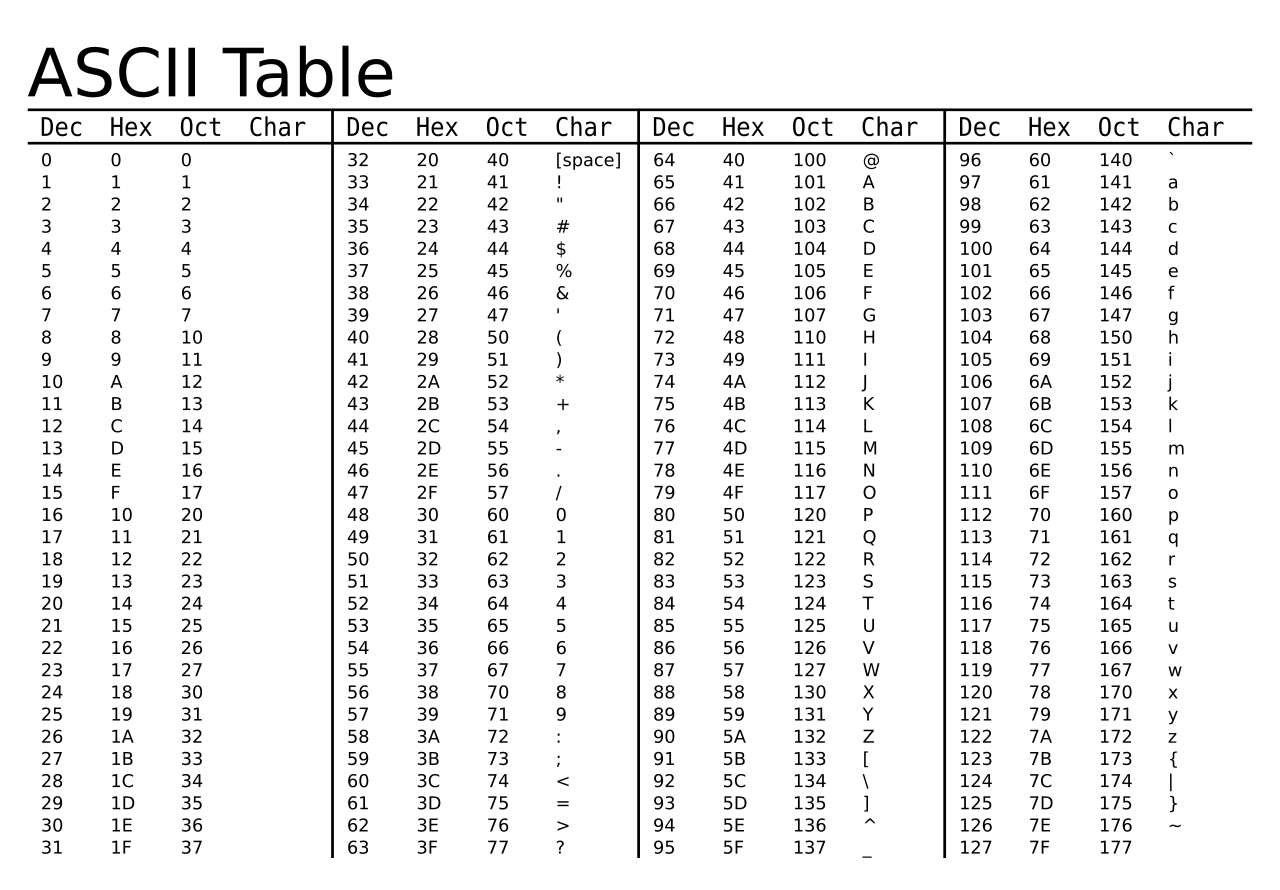
\includegraphics[width=\linewidth]{figures/outros/Ascii_Table.png}
\end{center}

\subsection{C++ Limits}
\begin{center}
  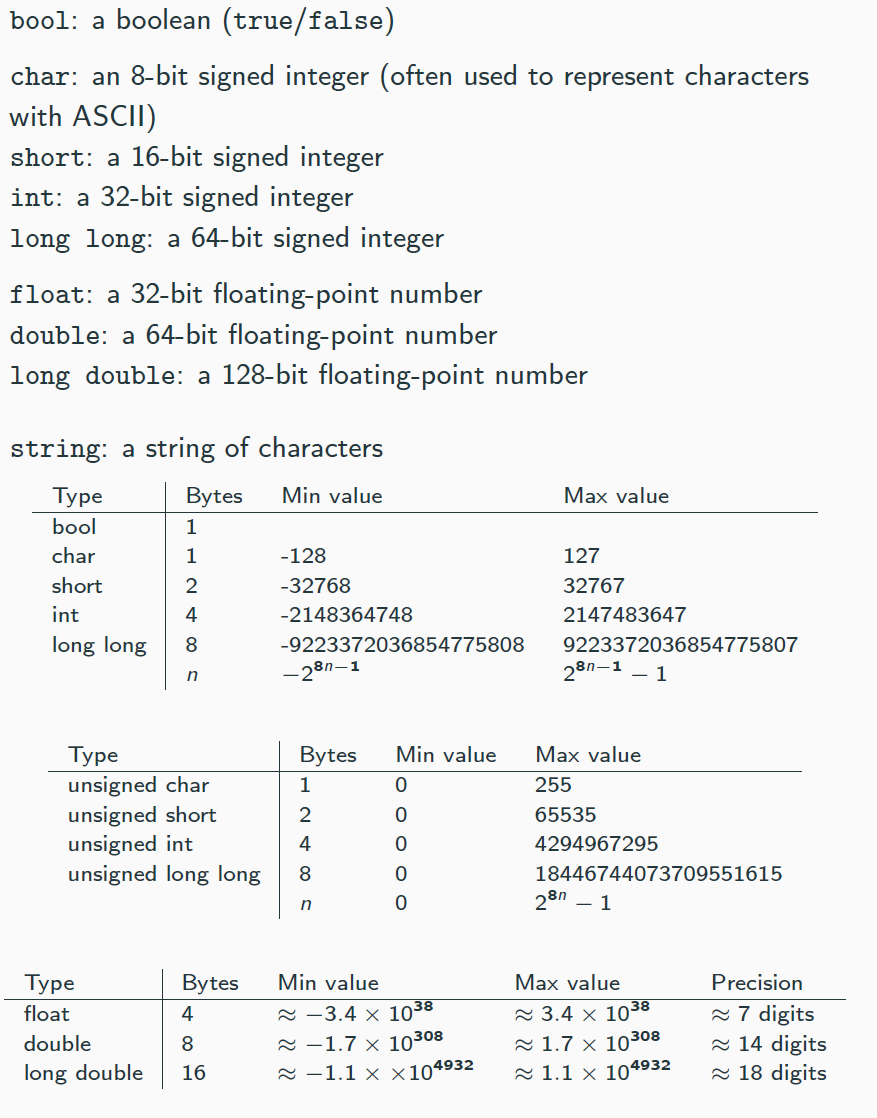
\includegraphics[width=\linewidth]{figures/outros/cpp_limits.png}
\end{center}

\subsection{Estruturas de dados C++}
\begin{center}
  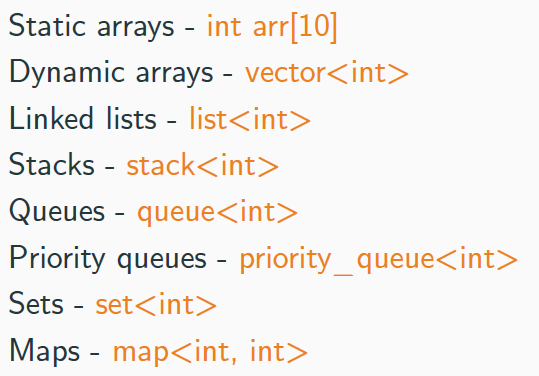
\includegraphics[width=\linewidth/2]{figures/outros/eds_c++.png}
\end{center}

\subsection{Conversão para números romanos}
\noindent Fazer teste com 444 IX IV CM CD XC XL. Lembre-se que I representa 1, V é 5, X é 10, L é 50, C é 100, D é 500 e M 1000

\subsection{Antes e depois de cristo}
\noindent Não existe ano 0, existe 1 A.C. e 1 D.C.

\subsection{Problemas que envolvem horário}
\noindent Procurar sempre usar minutos/segundos

\subsection{Ano bissexto}
\noindent Considerar 366 dias

\subsection{Ano normal}
\noindent Considerar 365 dias

\subsection{Dias de cada mês}
\noindent Janeiro(1) 31
\newline\noindent Fevereiro(2) 28(29 bissexto)
\newline\noindent Março(3) 31
\newline\noindent Abril(4) 30
\newline\noindent Maio(5) 31
\newline\noindent Junho(6) 30
\newline\noindent Julho(7) 31
\newline\noindent Agosto(8) 31
\newline\noindent Setembro(9) 30
\newline\noindent Outubro(10) 31
\newline\noindent Novembro(11) 30
\newline\noindent Dezembro(12) 31
\newline\noindent 30: 4 | 31: 7 | *28: 1 | *29: 1

\subsection{Número de letras no alfabeto}
\noindent 26, contando K, W e Y

\subsection{Forma alternativa para escrita de nome para tipos de dados}
\inserircodigo{c++}{outros/formas_escrever_tipos_dados.cpp}{8}{8}{}

\subsection{Inicializar vetor com valor predefinido}
\inserircodigo{c++}{outros/inicializar_vetor_com_valor_predefinido.cpp}{8}{8}{}

\subsection{Operações para modificar sequências}
\inserircodigo{c++}{outros/operacoes_para_modificar_sequencias.cpp}{8}{8}{}

\subsection{Permutações}
\inserircodigo{c++}{outros/permutacoes.cpp}{8}{8}{}

\subsection{Gerar números aleatórios}
\inserircodigo{c++}{outros/gerar_numeros_aleatorios.cpp}{8}{8}{}

\subsection{Pesquisa binária}
\inserircodigo{c++}{outros/busca_binaria.cpp}{8}{8}{}

\end{document}